\section{Computational Setup}

%!% Make this a script and do it for more cores....
\begin{figure}[h!tb]
  \centering
  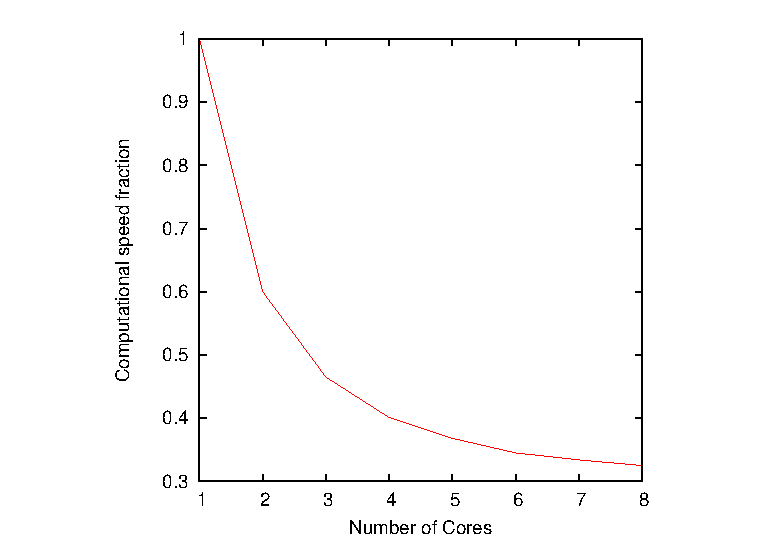
\includegraphics[scale=0.9]{corespeed.eps}
  \caption{Computation speed of simulations ran with different number of cores.
    The $y$-axis represents the fraction of time each core has in comparison to the the $1$-core result.
    Same simulation setup as the travelling wave simulation.
    Ran until $t = 2$ with a grid of $2049 \times 2049$. }
  \label{fig:corespeed}
\end{figure}

The implementation of Algorithm \ref{alg:iterateCM} was done with Fortran. 
The system is stored in diagonal format, since $A$ has five distinct diagonals.

All the computations were run on a custom built workstation with an Intel Xeon CPU E5-2650 (1.2 GHz, 20MB cache size) and 32 GB RAM under Red Hat Enterprise Linux Server release 6.5 (Santiago). 
Running the computations with OpenMP, took advantage of 4 out of the 16 threads of the Intel Xeon CPU, with 2 threads to each core.
The choice of 4 cores is because there is not enough computational gain from using extra, as shown in Figure \ref{fig:corespeed}.
The selection of 4 threads is because the computation time decrease becomes less efficient after more then 4 threads. 
The GNU Fortran compiler, version 4.4.7, was used for all computations; the compiler arguments were
\begin{verbatim} -03 -fdefault-real-8 -fopenmp \end{verbatim}



%!% Add other computers nd compilers to show that it was rigerously tested...
